\documentclass{standalone}
\usepackage{tikz}
\usetikzlibrary{shapes}
\usetikzlibrary{positioning}
\usepackage{amsmath}


%\tikzstyle{startstop} = [rectangle, rounded corners, text width=2cm,text centered, minimum height=1cm, draw=black]
\tikzstyle{io} = [trapezium, trapezium left angle=70,trapezium right angle=110, text width=3.5cm, minimum height=1cm, text centered, draw=black, trapezium stretches=true]
\tikzstyle{process} = [rectangle, text width=3.5cm, minimum height=1cm, text centered, draw=black]


\begin{document}
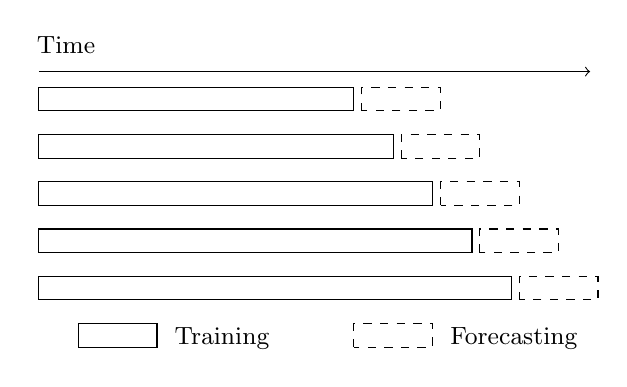
\begin{tikzpicture}

    % \node(start)[startstop]{Start};
    % \node(in)[io]{Input time series};

    % \node(rollingorigin)[process, right of=in]{Rolling origin transformation};
    % \draw [->](in.east) -- (rollingorigin.west) ;
    \node[anchor=south west] at (-0.15, 0.6) {\small Time};
    \draw[->] (0, 0.5) -- (7, 0.5);
    \draw[draw=black] (0, 0) rectangle ++(4, 0.3);
    \draw[draw=black, dashed] (4.1, 0) rectangle ++(1, 0.3);

    \draw[draw=black] (0, -0.6) rectangle ++(4.5, 0.3);
    \draw[draw=black, dashed] (4.6, -0.6) rectangle ++(1, 0.3);

    \draw[draw=black] (0, -1.2) rectangle ++(5, 0.3);
    \draw[draw=black, dashed] (5.1, -1.2) rectangle ++(1, 0.3);

    \draw[draw=black] (0, -1.8) rectangle ++(5.5, 0.3);
    \draw[draw=black, dashed] (5.6, -1.8) rectangle ++(1, 0.3);

    % \node[text centered,anchor=south west, minimum height=0.3] at (0, -2.4) {\large $\dots$};

    \draw[draw=black] (0, -2.4) rectangle ++(6, 0.3);
    \draw[draw=black, dashed] (6.1, -2.4) rectangle ++(1, 0.3);

    % \draw[draw=black] (0, -3) rectangle ++(6.5, 0.3);
    % \draw[draw=black, dashed] (6.6, -3) rectangle ++(1, 0.3);

    \draw[draw=black] (0.5, -3) rectangle ++(1, 0.3);
    \node[anchor=south west] at (1.6, -3.15) {\small Training};

    \draw[draw=black, dashed] (4, -3) rectangle ++(1, 0.3);
    \node[anchor=south west] at (5.1, -3.15) {\small Forecasting};

    % \node(train1)[process, above right = 1cm and 0.75cm of rollingorigin, ]{Obtain $h$-step-ahead forecasts for each window};
    % \draw[->] (rollingorigin.north) |- (train1.west) ;
    % \node(train2)[process, right of=rollingorigin]{Obtain $h$-step-ahead realization for each window};
    % \draw[->] (rollingorigin.east) -- (train2.west) ;
    % \node(train3)[process, right of=train2]{Train reconciliation matrix $A_1,\dots,A_h$};
    % \draw[->] (train2.east) -- (train3.west);
    % \draw[->] (train1.east) -| (train3.north);

    % \node(forecast1)[process,below right = 1cm and 0.75cm of rollingorigin]{Obtain $h$-step-ahead base forecasts $\hat{\mathbf{\pi}}_{T+1},\dots,\hat{\mathbf{\pi}}_{T+h}$};
    % \draw[->] (rollingorigin.south) |- (forecast1) ;
    % \node(forecast2)[process, right of=forecast1]{Obtain $h$-step-ahead reconciled distribution};
    % \draw[->] (forecast1) -- (forecast2);
    % \node(output)[io, right of=forecast2]{Output coherent forecast $\tilde{\mathbf{\pi}}_{T+1},\dots,\tilde{\mathbf{\pi}}_{T+h}$};
    % % % \node(end)[startstop, below of=output]{End};

    % % \draw[->] (start) edge (in)
    % 
    % 

    % \draw[->] (train1) |- (train3);
    % %\draw[->] (in.east) -| (forecast1.north);
    % \draw[->] (train3.south) -- (forecast2.north);
    % \draw[->] (forecast2) -- (output);
    % 


    % \draw[->] (forecast2) -- (output);
    % \draw[->] (output) -- (end);

\end{tikzpicture}
\end{document}
